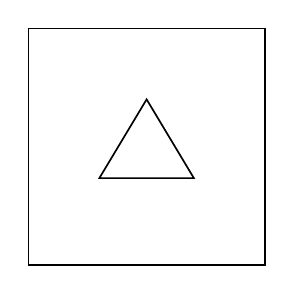
\begin{tikzpicture}[x=1cm,y=1cm,font=\normalsize,
 geometry edge/.style={solid,line width=.6pt},
 geometry mark/.style={solid,line width=.6pt},
 geometry label/.style={font=\normalsize,inner sep=2pt}]
\coordinate (G1) at (-1.5,-1.5);
\coordinate (G2) at (1.5,-1.5);
\coordinate (G3) at (1.5,1.5);
\coordinate (G4) at (-1.5,1.5);
\coordinate (H1) at (0,0.6);
\coordinate (H2) at (-0.6,-0.4);
\coordinate (H3) at (0.6,-0.4);
\draw[geometry edge] (G1)--(G2)--(G3)--(G4)--cycle;
\draw[geometry edge] (H1)--(H2)--(H3)--cycle;
\end{tikzpicture}
